% Copyright (c) 2019 Jiazheng Li. All rights reserved.
% Author: Jizheng Li

\documentclass[UTF8,11pt]{beamer}
\usepackage{talkbeamer}


\title[如何使用\LaTeX 排版]{\LaTeX 入门简介}
\subtitle{如何使用\LaTeX 排版}
\author{李嘉政}
\date{\today}
%\institute{东北电力大学}


\begin{document}

\begin{frame}
    \titlepage
\end{frame}

\begin{frame}{目录}
	\tableofcontents
	% [pausesections]
\end{frame}


\section{简介}
\subsection{\TeX 与 \LaTeX}
\begin{frame}{\TeX 与 \LaTeX}
	\begin{columns}
		\column{8cm}
		\begin{enumerate}
		\item \TeX \quad(/'t\textepsilon k/,/'t\textepsilon x/)
		\begin{itemize}
			\item 最初由Donald E. Knuth于 1978 年开发
			\item 生成精美的图书排版系统
			\item 漂亮、美观、稳定、通用
			\item 尤其擅长数学公式的排版
			\item 当前的版本号为 \TeX \; 3.14159265
		\end{itemize}
		\item \LaTeX \quad(/'leit\textepsilon k/)
		\begin{itemize}
			\item Leslie Lamport开发\LaTeX 降低使用门槛
			% \item 每一个LaTeX 命令实际上最后都会被转换解释成几个甚至上百个TeX 命令。
			\item 最流行和使用最为广泛的\TeX 宏集
			\item 广泛用于学术界,期刊会议论文模板
			\item 大学学位论文模板
			\item CV、Poster
		\end{itemize}
		\end{enumerate}
	\column{6cm}
	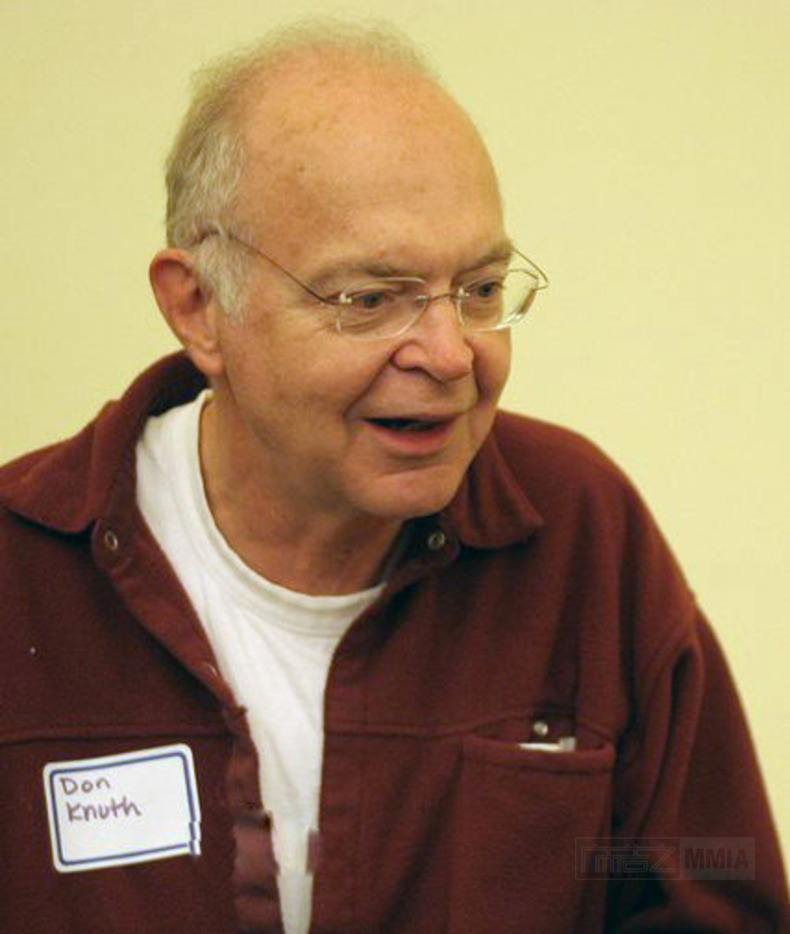
\includegraphics[scale=0.15]{figure/DK}\\
	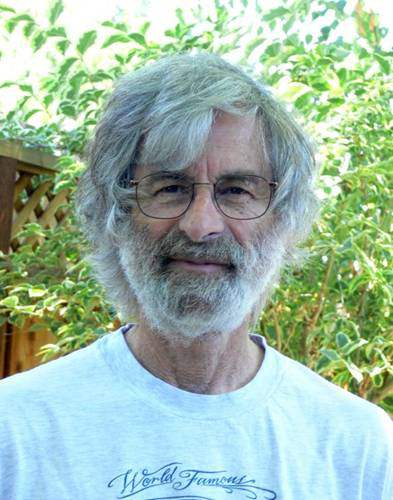
\includegraphics[scale=0.28]{figure/LL}
	\end{columns}
\end{frame}

\begin{frame}{几个概念}
	\begin{description}
		\item[套装发行版] :是\TeX 排版引擎、支持排版的文件( 基本格式、 \LaTeX 宏包、字体等)以及一些辅助工具的集合。
			\begin{itemize}
				\item {\color{red}\TeX \,Live}:TUG开发,跨平台,更新及时,值得信赖
				\item {\color{red}Mik\TeX}:Windows专享,宏包安装方便,值得信赖
				\item {\color{red}Mac\TeX}:虽然我买不起苹果电脑,但是仍然值得信赖
				\item {\color{red}CTeX}:不推荐,但是想用还是可以用的,开心就好。
			\end{itemize}
		\item[编辑器] :用什么东西写代码
		\begin{itemize}
			\item 专用免费编辑器:TeXworks、TeXStudio、TeXmaker
			\item 专用收费编辑器:WinEdt
			\item 通用文本编辑器:Vim、VS Code、Sublime、Atom
			\item 其他:Notepad
		\end{itemize}	
	\end{description}

	
\end{frame}
\begin{frame}{\TeX 编译引擎}
	\begin{enumerate}
		\item \TeX (latex):tex->dvi->pdf (需要其他工具)
		\item \pdfTeX (pdflatex):tex->pdf (不支持Unicode,西文首选)
		\item \LuaTeX (lualatex):tex->pdf (支持Unicode,但不稳定)
		\item \XeTeX (xelatex):tex->xdv->pdf (支持Unicode,中文首选)
		\item \BibTeX (bibtex):输出参考文献
	\end{enumerate}
	\bfseries CTeX套装发行版和\CTeX 宏包/文档类是两回事,请使用\CTeX 宏包配合UTF-8编码进行中文排版!
\end{frame}

\subsection{和Word对比}
\begin{frame}{和word对比}
	\begin{center}
		\begin{tabular}{c|c}
			\hline
			Microsoft\textsuperscript{\textregistered}word & \LaTeX \\
			\hline
			\rowcolor{black!20}
			文字处理工具			& 专业排版软件  \\
			容易上手,简单直观 	  & 学习成本高   \\
			\rowcolor{gray!40}
			所见即所得			 & 所见即所想,所想即所得  \\
			高级功能不易掌握 	   & 进阶难,但一般用不到  \\
			\rowcolor{gray!40}
			需要花费大量时间调格式	& 专心内容,无需关系格式 \\
			公式排版差强人意	  & 尤其擅长公式排版 \\
			\rowcolor{gray!40}
			各版本兼容性差		  & 易读,稳定 \\
			商业付费			& 开源免费 \\
			\hline
		\end{tabular}	
	\end{center}
\end{frame}

\begin{frame}{不要陷入这三个坑}
	\begin{enumerate}
		\item 请远离CJK宏包与CTeX套装
		\begin{itemize}
			\item CJK是十年前处理中文的方式
			\item CTeX套装已经多年未更新,功能较为冗余
			\item 处理中文,优先使用\CTeX 宏包或xeCJK宏包
		\end{itemize}
		\item 不要按Word的思路来学习/使用\LaTeX
		\begin{itemize}
			\item 常见误区:强制换行、更换字体、图文混排
			\item "怎样在\LaTeX 中实现Word中的xx功能"
			\item 请逐渐习惯\LaTeX 的思维方式
		\end{itemize}
		\item 切勿花费过多精力于\LaTeX 的细枝末节上
		\begin{itemize}
			\item \TeX/\LaTeX 是进四十年前的发明,与现代程序设计原理有所冲突
			\item 四十年来的层层累进,内容太多,不要指望能够马上学会
			\item 文档的内容最重要
			\item 使用\LaTeX 的最高境界:拍好内容且不浪费时间
		\end{itemize}
	\end{enumerate}
	
\end{frame}



\subsection{\TeX 排版举例}\label{eq_example}
\begin{frame}{\TeX 排版举例:数学公式}
	\begin{block}{无编号公式}
		$$ f(x)=f(x^{(0)})+f^{'}(x^{(0)})\Delta +\frac{1}{2}f^{''}(x^{(0)})(\Delta x)^2+\cdots$$
	\end{block}
	
	\begin{block}{有编号公式}
		\begin{equation}\label{eq1}
			f(x) = 
			\begin{cases}
			\dfrac{\cos{x}}{x+\sin{x}} & x \geq 0 \\
							ax^2+bx+c & x \leq 0
			\end{cases}
		\end{equation}
		\begin{equation}\label{eq2}
		 \lim_{x \rightarrow 0} \frac{\sin x}{x}=1
		\end{equation}
	\end{block}
\end{frame}


\begin{frame}{\TeX 排版举例:数学公式}
	\begin{block}{矩阵}
		$$	A=\begin{bmatrix} \frac{\partial^2f }{\partial x_1^2} &\frac{\partial^2 f}{\partial x_1 \partial x_2} & \cdots & \frac{\partial^2f}{\partial x_1\partial x_n}\\ \frac{\partial^2f}{\partial x_2\partial x_1 } & \frac{\partial^2f}{\partial x_2^2}&\cdots &\frac{\partial^2f}{\partial x_2\partial x_n} \\\vdots&\vdots&\ddots & \vdots\\ \frac{\partial^2f}{\partial x_n\partial x_1}&\frac{\partial^2f}{\partial x_n \partial x_2}&\cdots&\frac{\partial^2f }{\partial x_n^2}  \end{bmatrix}$$		
	\end{block}
	\begin{block}{花体字}
		$$\mathbb{ABCDEFGHIJKLMNOPQRSTUVWXYZ}$$
		$$\mathscr{ABCDEFGHIJKLMNOPQRSTUVWXYZ}$$ 
		$$\mathcal{ABCDEFGHIJKLMNOPQRSTUVWXYZ}$$
	\end{block}
\end{frame}


\begin{frame}{\TeX 排版举例:图形排版}
	\begin{columns}[c]  %开始进入分栏环境,居中设置
		\column{7cm}
	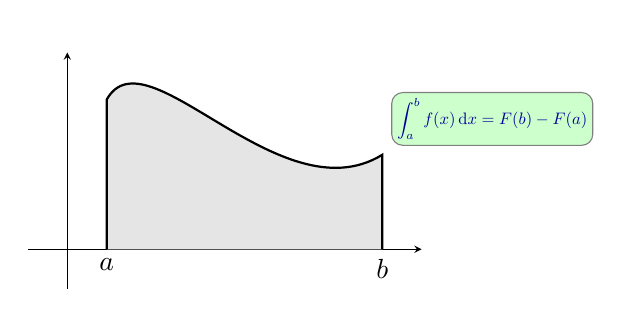
\begin{tikzpicture}
	\draw[-stealth,line width=0.2pt] (-0.5,0) -- (4.5,0);
	\draw[-stealth,line width=0.2pt] (0,-0.5) -- (0,2.5);
	\coordinate (a) at (0.5,1.9);
	\coordinate (b) at (4,1.2);
	\node[below] (a0) at (a |- 0,0) {$a$};
	\node[below] (b0) at (b |- 0,0) {$b$};
	\filldraw[fill=gray!20,draw,thick]
	(a0) -- (a) .. controls (1,2.8) and (2.7,0.4) .. (b) -- (b0) -- cycle;
	\node[above right,outer sep=0.2cm, rounded corners,
	fill=green!20,draw=gray,text=blue!60!black,scale=0.6]
	at (b) {$\displaystyle \int_a^b {f(x)\,\mathrm{d}x} = F(b) - F(a)$};
	\end{tikzpicture}
	
	\column{4cm}
	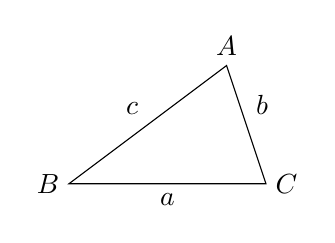
\begin{tikzpicture}
	\draw (2,1.5) node[above] {$A$}
	-- node[above left] {$c$}
	(0,0) node[left] {$B$}
	-- node[below] {$a$}
	(2.5,0) node[right] {$C$}
	-- node[above right] {$b$}
	cycle;
	\end{tikzpicture}
	\end{columns}
\end{frame}

\begin{frame}{\TeX 排版举例:算法}
\begin{figure}
	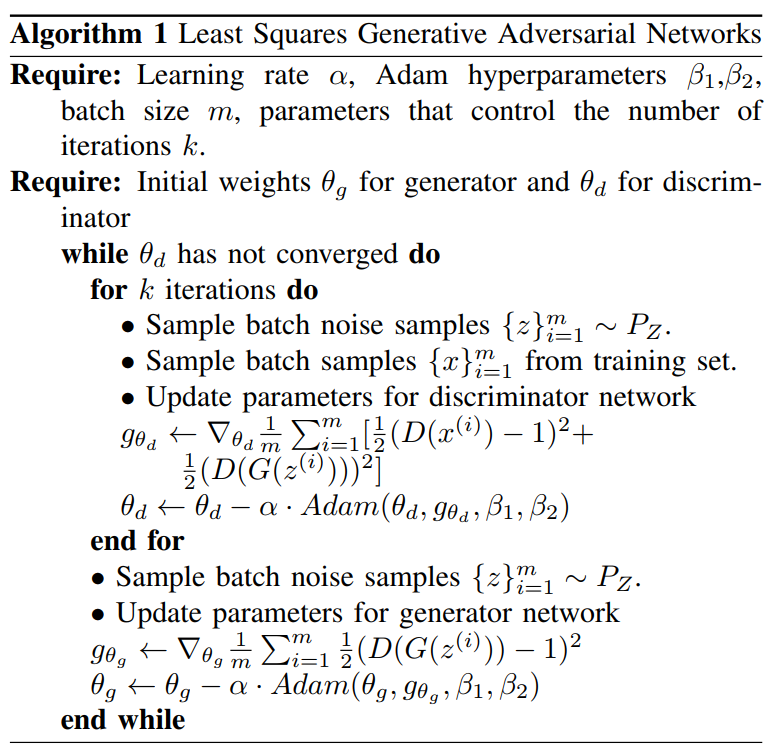
\includegraphics[scale=0.4]{figure/Algorithm.png}
\end{figure}
\end{frame}

\begin{frame}{\TeX 排版举例:文档}
	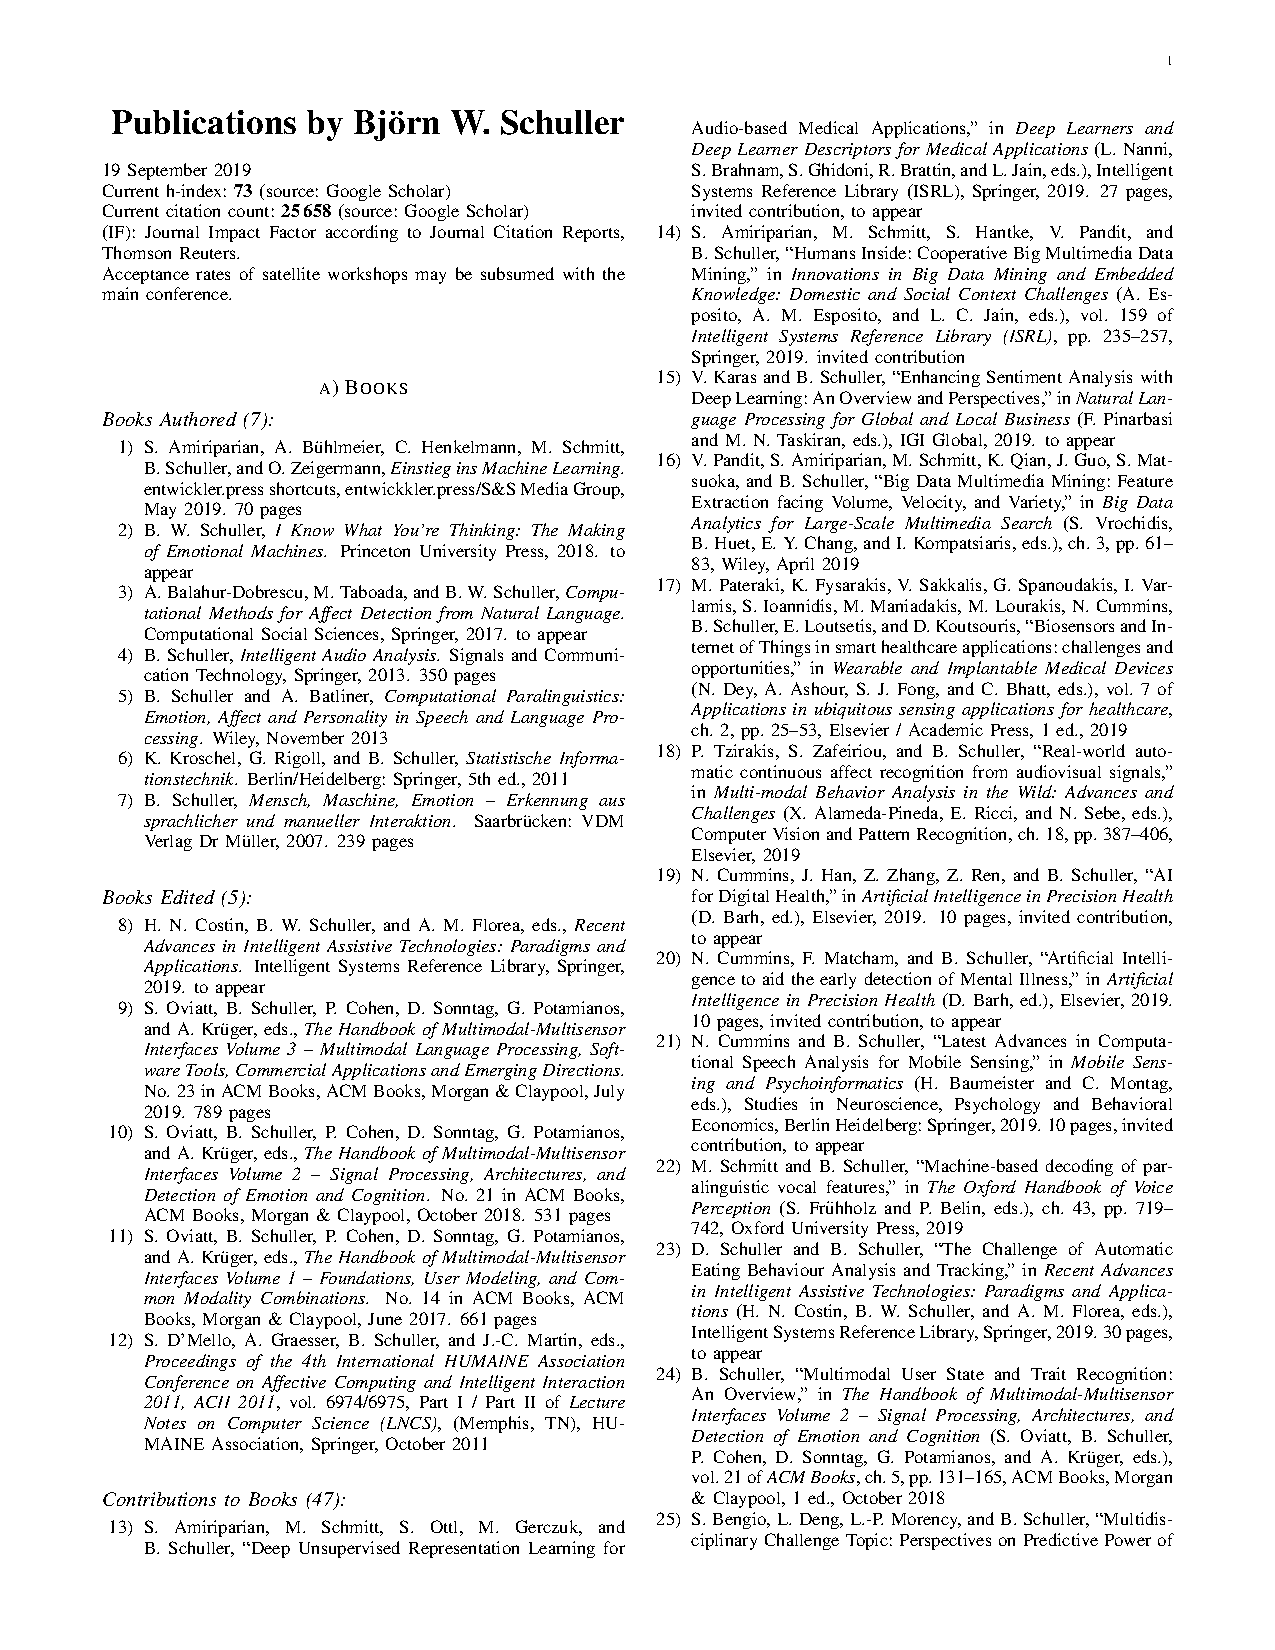
\includegraphics[scale=0.25]{figure/bib}
	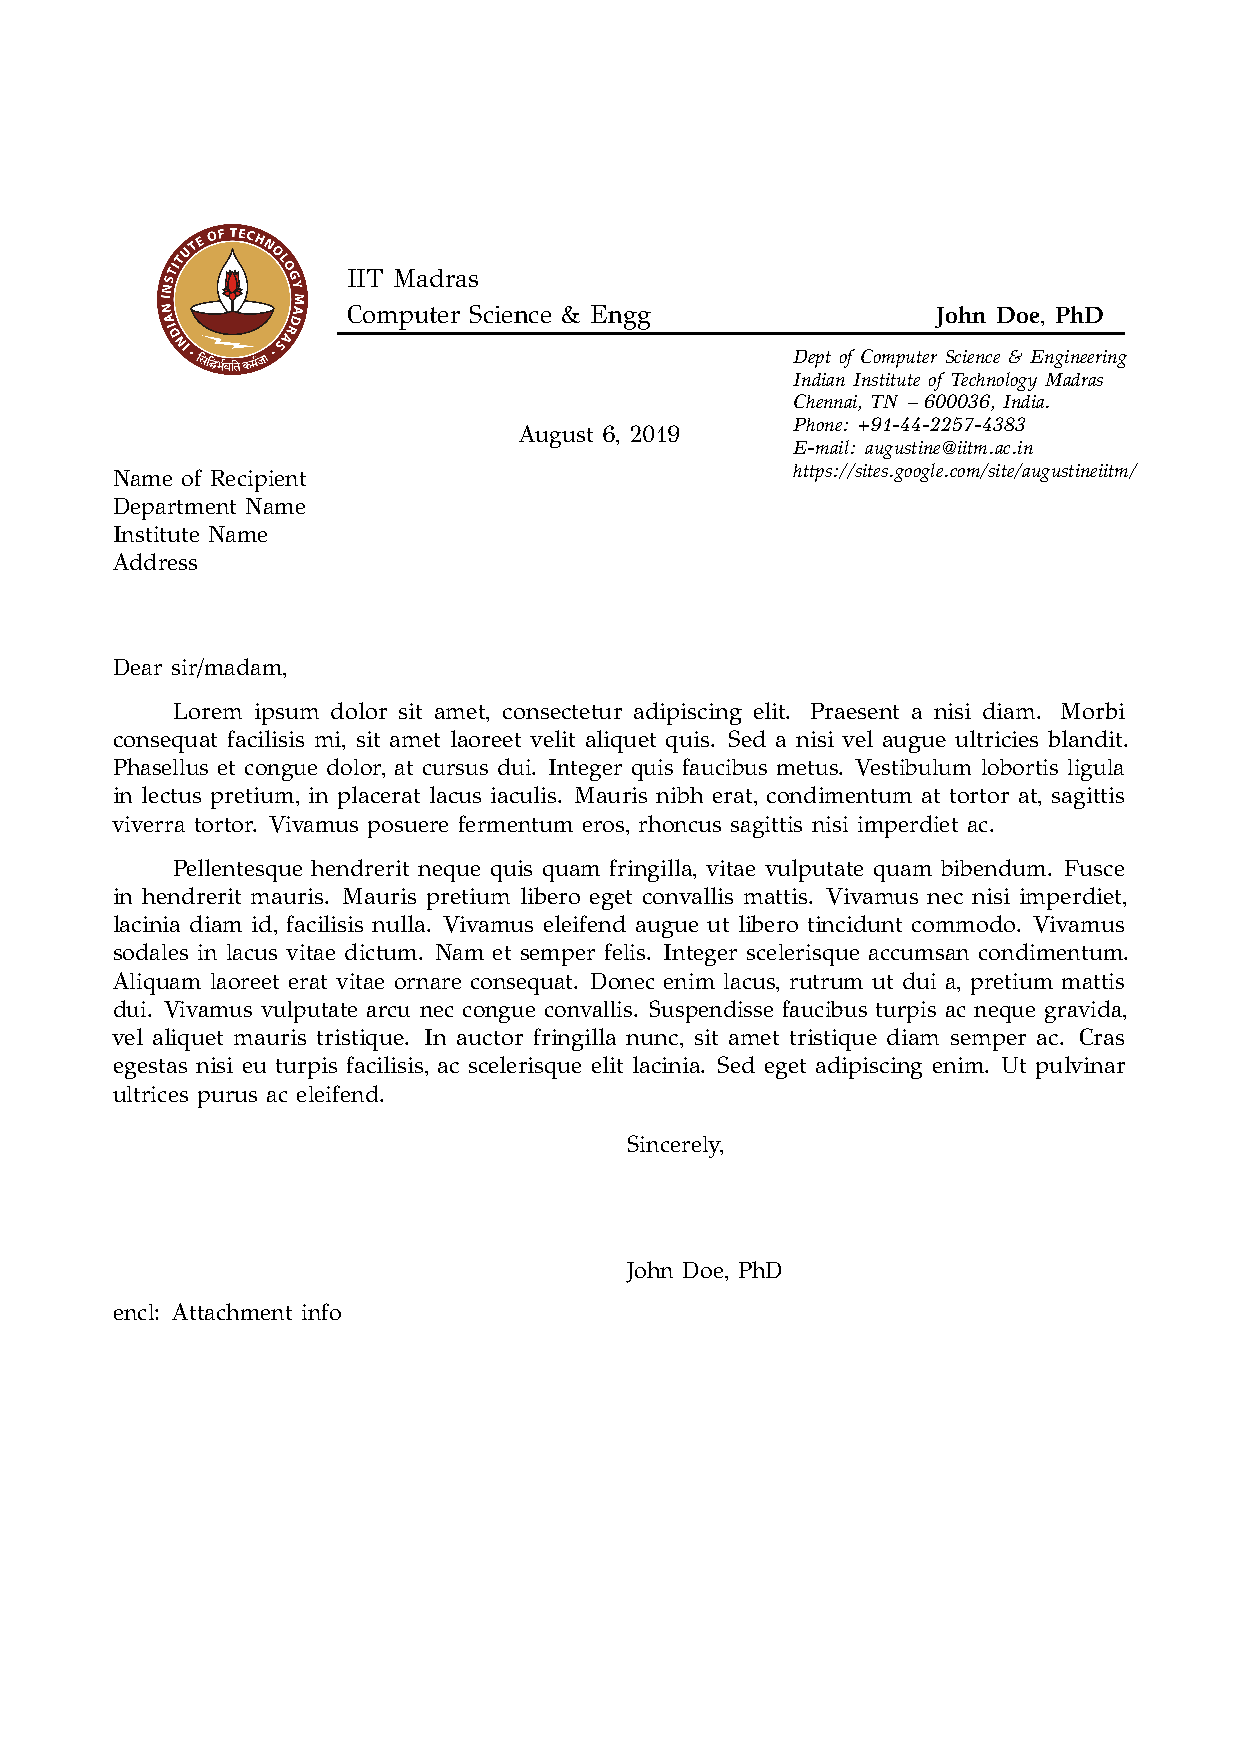
\includegraphics[scale=0.25]{figure/letter}
\end{frame}


\begin{frame}{\TeX 排版举例:文档}
	\centering
	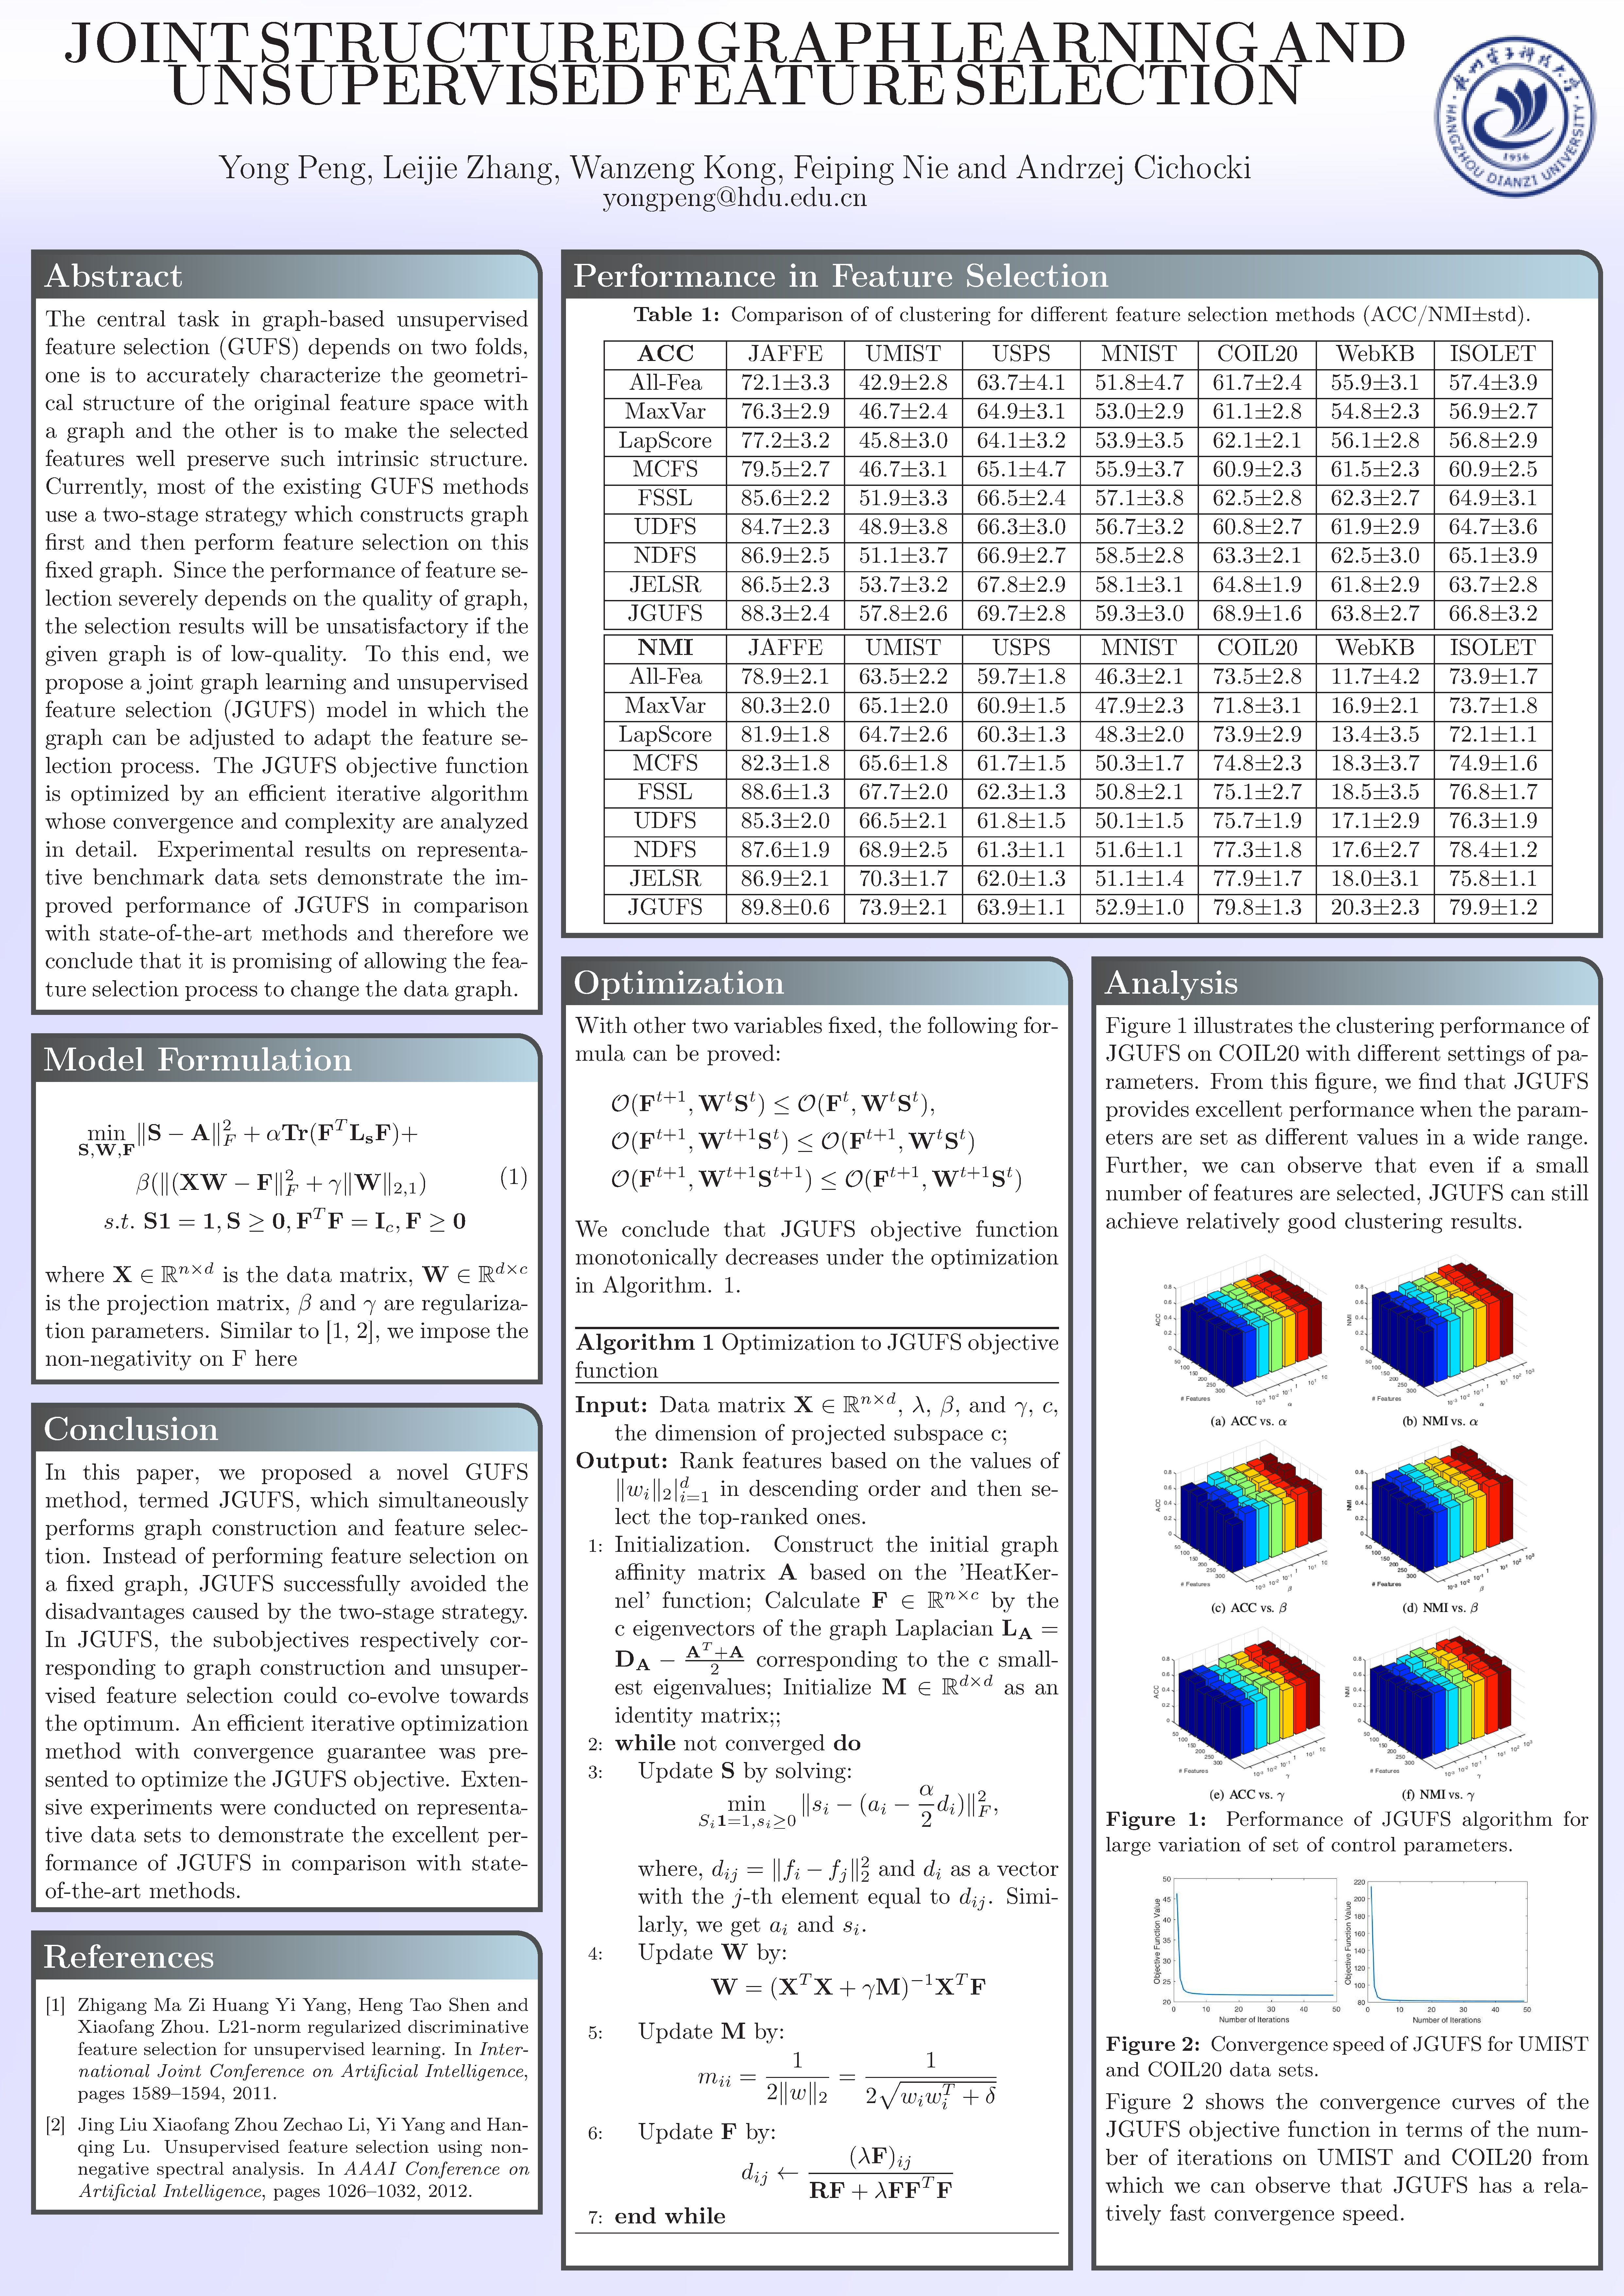
\includegraphics[width=5.5cm,height=8cm]{figure/poster}
\end{frame}


\begin{frame}{\TeX 排版举例:文档}
	\centering
	
\includegraphics[width=5.5cm,height=7.5cm]{figure/book}
\end{frame}


\begin{frame}{\TeX 排版举例:幻灯片}
	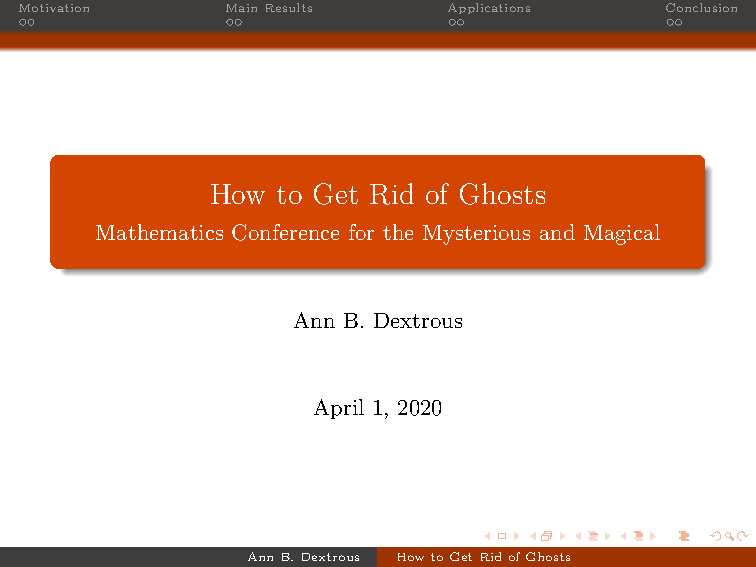
\includegraphics[scale=0.45]{figure/examplebeamer1}
	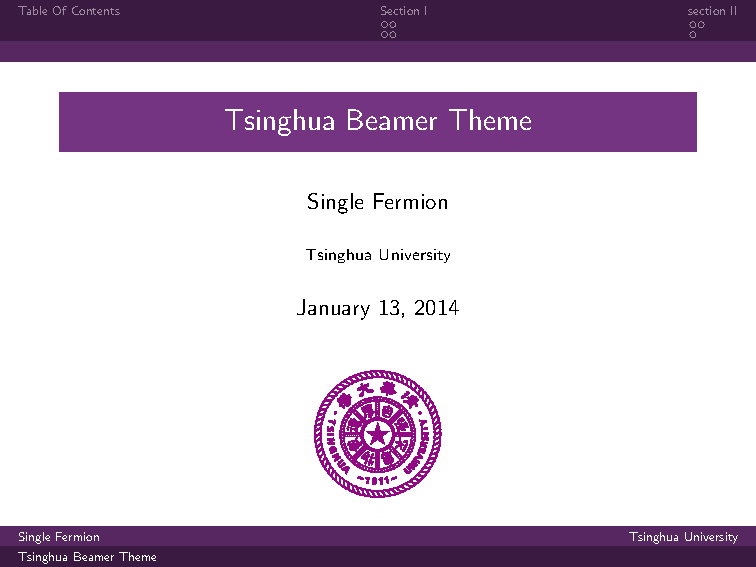
\includegraphics[scale=0.45]{figure/examplebeamer2}
\end{frame}



\section{排版}

\subsection{\LaTeX 排版入门}
\begin{frame}[fragile]
	\frametitle{基本结构}
	\begin{lstlisting}
%% 导言区
\documentclass[11pt,utf8]{article} %report,book,beamer
\usepackage{ctex}  % 中文支持宏包
\title{一篇不太简短的\LaTeXe 简介}
\author{Tobias Oetiker}
\date{\today}

%% 正文区
\begin{document} 
\maketitle % 自动生成标题页
这里是正文
\end{document} 
\end{lstlisting}
\end{frame}

\begin{frame}[fragile]{宏包与环境}	
	在使用 \LaTeX 时,时常需要依赖一些扩展来增强或补充\LaTeX 的功能,比如排版复杂的表
	格、插入图片、增加颜色甚至超链接等等。这些扩展称为宏包。
\begin{lstlisting}
\usepackage{package}
\end{lstlisting}
\LaTeX 还引入了环境的用法,用以令一些效果在局部生效,或是生成特殊的文档元素。 
\begin{lstlisting}	
\begin{<environment name>}{<arguments>}
. . .
\end{<environment name>}
\end{lstlisting}
\end{frame}


\begin{frame}{\LaTeX 命令}	
	\begin{enumerate}[<+-| alert@+>]
		\item 简单命令:\textbackslash 命令
		\begin{itemize}
			\item  \{\textbackslash songti 东北电力大学\} $\rightarrow$ {\songti 东北电力大学}
			\item \textbackslash zihao\{2\}电气工程学院 $\rightarrow$ {\zihao{2}电气工程学院} 
			
			\item \textbackslash Large\textbackslash textbf\{我最帅\} $\rightarrow$ \Large\textbf{我最帅}
		\end{itemize}
		\item 环境
		\begin{itemize}
			\item 无序列表环境 \textbackslash begin\{itemize\} ... \textbackslash end\{itemize\}
			\item 有序列表环境 \textbackslash begin\{enumerate\} ... \textbackslash end\{enumerate\}
		\end{itemize}
	\end{enumerate}
\end{frame}

\begin{frame}[fragile]{\LaTeX 环境命令举例}
	\begin{columns}[c]
		\column{7cm}
		\begin{lstlisting}
\begin{itemize}
\item 第一
\item 第二
\item 第三
\end{itemize}
\end{lstlisting}
		\column{7cm}
		\begin{itemize}
			\item 第一
			\item 第二
			\item 第三
		\end{itemize}
	\end{columns}	
	
	\begin{columns}[c]
		\column{7cm}
\begin{lstlisting}
\begin{enumerate}
\item 绝对不意气用事
\item 绝对不漏判任何一件坏事
\item 绝对裁判的公正漂亮
\end{enumerate}
\end{lstlisting}
		\column{7cm}
		\begin{enumerate}
			\item 绝对不意气用事
			\item 绝对不漏判任何一件坏事
			\item 绝对裁判的公正漂亮
		\end{enumerate}
	\end{columns}
\end{frame}


\begin{frame}{\LaTeX 环境命令举例}
	\begin{block}{常用命令}
		\begin{center}
			\begin{tabular}{llll}
			\textbackslash chapter & \textbackslash section & \textbackslash maketitle & \textbackslash tableofcontents  \\ 
			章 & 节 & 生成标题页 & 生成目录 \\ \cline{1-4}
			\textbackslash newpage & \textbackslash makebox & \textbackslash vskip & \textbackslash caption \\
			新的一页 & 生成盒子 & 垂直距离 & 标题 \\ \cline{1-4}
			\textbackslash label & \textbackslash ref & \textbackslash includegraphics & \textbackslash cite \\
			标号 & 引用图表公式等 & 插入图片 & 引用参考文献
			
			\end{tabular}
		\end{center}
	\end{block}
\end{frame}

\begin{frame}[fragile]{文章结构}
	\begin{columns}
		\column{7cm}
\begin{lstlisting}
\usepackage{ctex}
\tableofcontents % 生成目录
\chapter{有监督学习}
\section{分类}
\subsection{逻辑回归}
\section{回归}
\subsection{线性回归}
\end{lstlisting}
		\column{7cm}
	
\includegraphics[scale=0.4]{figure/text}
	\end{columns}
\end{frame}


\begin{frame}[fragile]{交叉引用和脚注}
	\begin{columns}
		\column{7cm}
\begin{lstlisting}
% 给对象命名:图片、表格、公式 
\label{key} 
% 引用对象  
\ref{label} 
\pageref{label}
\end{lstlisting}
	\column{5cm}	
从第\pageref{eq_example} 页的公式 \ref{eq1} 中我们可以看出
	\end{columns}
	\begin{columns}
		\column{7cm}
\begin{lstlisting}
\footnote{text}
\end{lstlisting}
		\column{5cm}
		这里有一个可爱的脚注\footnote[frame]{我在这里}
	\end{columns}
\end{frame}


\begin{frame}[fragile]{交叉引用和脚注}
	\begin{columns}
		\column{7cm}
\begin{lstlisting}
东电图标请参见图~\ref{fig:logo}
\begin{figure}[htbp]
\centering
\includegraphics[scale=0.08]%
{figure/neepu_logo}
\caption{东北电力大学图标}
\label{fig:logo}
\end{figure}
\end{lstlisting}
		\column{6cm}
		\centering
		东电图标请参见图~\ref{fig:logo}	
		\begin{figure}[htbp]
			
\includegraphics[scale=0.08]{figure/neepu_logo}
			\caption{东北电力大学图标}
			\label{fig:logo}
		\end{figure}
	\end{columns}
\end{frame}

\begin{frame}[fragile]{参考文献}
	\begin{columns}
		\column{6cm}
		LaTeX提供了\textbackslash cite 命令用于引用参考文献:
\begin{lstlisting}
\cite{<citation>}
\end{lstlisting}
	 \begin{itemize}
		\item 推荐使用\BibTeX 样式
			\begin{itemize}
				\item 参考文献自动管理
				\item bib文件
				\item bst参考文献样式
			\end{itemize}
		\end{itemize}
\begin{lstlisting}
在许多文献\cite{li2018two,li2018optimal}中
\end{lstlisting}
		如“在许多文献\cite{li2018two,li2018optimal}中”
		\column{5cm}
		{\zihao{-6}
			
	@article\{li2018two,
	
	title=\{A two-stage approach for combined heat and power economic emission dispatch: Combining multi-objective optimization with integrated decision making\},

	author=\{Li, Yang and Wang, Jinlong and Zhao, Dongbo and Li, Guoqing and Chen, Chen\},
	
	journal=\{Energy\},
	
	volume=\{162\},
	
	pages=\{237--254\},
	
	year=\{2018\},

	publisher=\{Elsevier\}
\}
}
	\end{columns}     
\end{frame}

\begin{frame}{参考文献}
	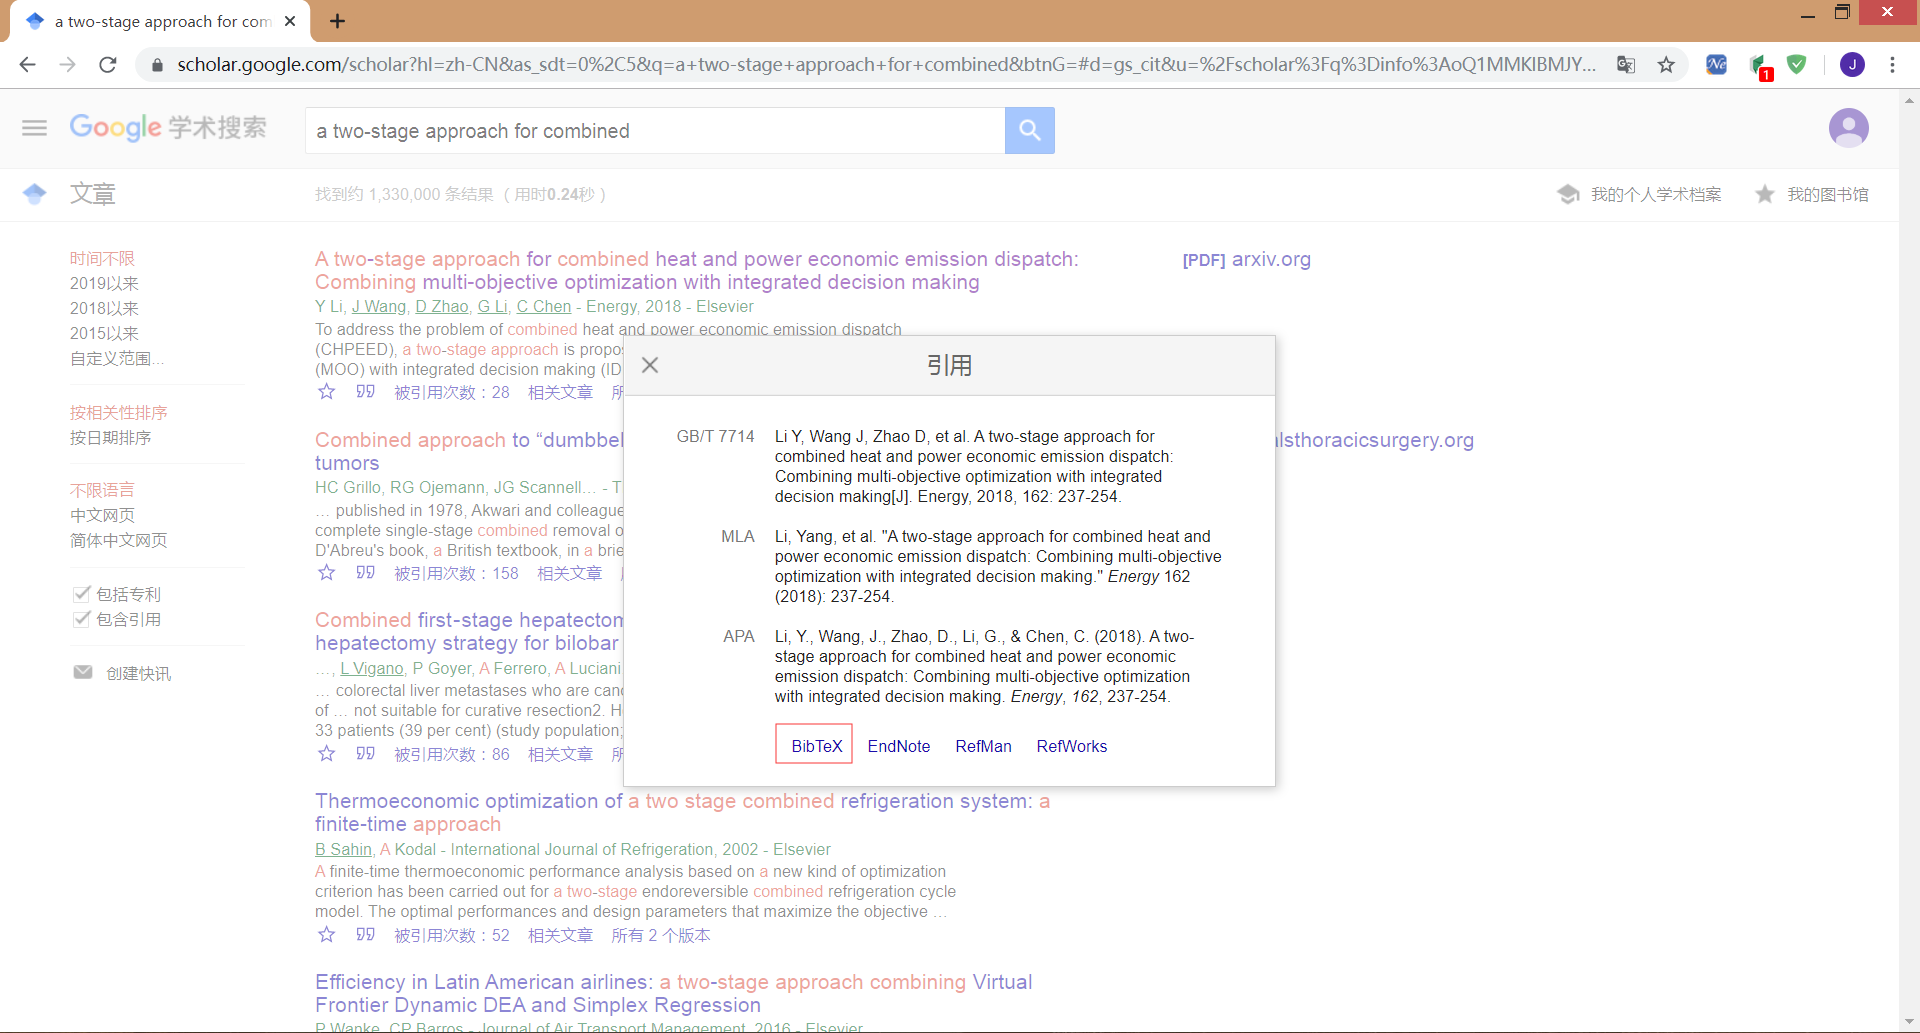
\includegraphics[scale=0.25]{figure/ref}
\end{frame}

\begin{frame}
	\frametitle{数学公式}
	数学公式排版是\LaTeX 的绝对强项,在\LaTeX 中排版数学公式需要进入数学模式
	\begin{itemize}
		\item 用两个\$美元符包围起来的是行内公式
		\item 用两个双美元符\$\$包围起来的是行间公式
		\item 用equation环境包围的是带编号的公式
		\item 条件公式用cases环境,多行公式用split、align、gather环境等
		\item 运行 texdoc symbols 查看符号表
	\end{itemize}
\end{frame}


\begin{frame}[fragile]
	\frametitle{数学公式}
\begin{lstlisting}
在公式$V = \frac{4}{3}\pi r^2$中,有:
$$\lim_{n \rightarrow \infty}(1+\frac{1}{n})^n=e \quad V = \frac{4}{3}\pi r^2$$
这是一个极限n趋于无穷大的极限
\end{lstlisting}

在公式$V = \frac{4}{3}\pi r^2$中,有:$$\lim_{n \rightarrow \infty}(1+\frac{1}{n})^n=e \quad V = \frac{4}{3}\pi r^2$$这是一个极限$n$趋于无穷大的极限
\end{frame}

\begin{frame}[fragile]
\begin{lstlisting}
$D$ and $G$ play the following two-player minimax game with value function $V (G; D)$:
\begin{equation}
\min_{G}\max_{D}V(G,D)=\mathbb{E}_{x\sim P_{data}}[\log D(x)]+\mathbb{E}_{z \sim P_{z}}[\log(1-D(G(z)))]
\end{equation}
\end{lstlisting}
$D$ and $G$ play the following two-player minimax game with value function $V (G; D)$:
\begin{equation}
	\min _{G} \max _{D} V(G,D)=\mathbb{E}_{x \sim P_{data}}[\log D(x)]+\mathbb{E}_{z \sim P_{z}}[\log (1-D(G(z)))]
\end{equation}
\end{frame}


\subsection{模板的使用}
\begin{frame}{排版}{模板的使用}
	\begin{itemize}[<+->]
		\item 模板
		\begin{itemize}
			\item[*] 已经设计好的格式框架
			\item[*] 不应将时间花费在调整框架上
		\end{itemize}
		\item 哪里获取模板
		\begin{itemize}
			\item[*] 上网下载
			\item[*] .cls文档类
			\item[*] .sty宏包 
		\end{itemize}
	\end{itemize}
\end{frame}

\begin{frame}[fragile]{IEEE \LaTeX Class}
\footnotesize
\begin{lstlisting}
\title{Optimal Scheduling of an Isolated Microgrid With Battery Storage Considering Load and Renewable Generation Uncertainties}
\author{Yang~Li,~\IEEEmembership{Member,~IEEE,}Zhen~Yang,Guoqing~Li,Dongbo~Zhao,~\IEEEmembership{Senior Member,~IEEE,} and Wei~Tian,~\IEEEmembership{Senior Member,~IEEE,}}
\maketitle
\end{lstlisting}
\begin{figure}
	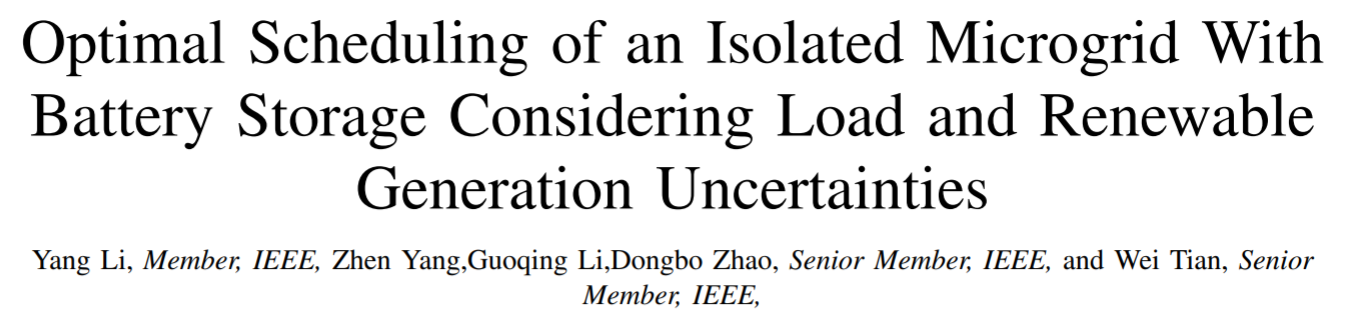
\includegraphics[scale=0.3]{figure/title.png}
\end{figure}
\end{frame}

\begin{frame}[fragile]
\scriptsize
\begin{lstlisting}
\begin{abstract}
abstract abstract abstract abstract abstract abstract abstract abstract
\end{abstract}
\begin{IEEEkeywords}
deep learning, microgird
\end{IEEEkeywords}
\section{INTRODUCTION}
\subsection{Literature Review}
\subsection{Contribution of This Paper}
\subsection{Organization of This Paper}
\section{UNCERTAINTY MODELING OF MICROGRIDS}
\subsection{Probabilistic WT Model}
\end{lstlisting}
\begin{figure}
	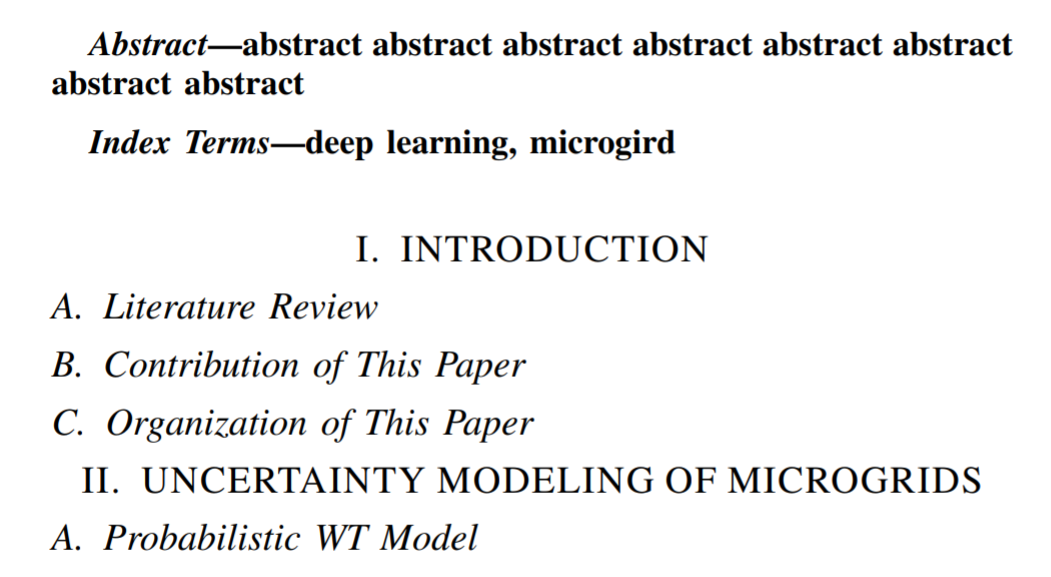
\includegraphics[scale=0.3]{figure/IEEE.png}
\end{figure}
\end{frame}


\section{总结}
\subsection{学习建议}
\begin{frame}{阅读材料}
	\begin{enumerate}
	\item 略读包太雷《 \LaTeX \;Notes(第二版)》
	\item 仔细阅读《 一份不太简短的 \LaTeXe 介绍》(lshort-zh)
	\item 仔细阅读\CTeX 宏集手册
	\item \LaTeX 入门(刘海洋)
	\item 根据所需宏包查阅宏包手册
	\item texdoc 例如: texdoc lshort-zh
	\end{enumerate}
\end{frame}




\subsection{\LaTeX 网站}
\begin{frame}{\LaTeX 网站}
	\begin{columns}
		\column{5cm}
	\begin{itemize}
	\item \href{https://www.overleaf.com}{Overleaf}
	\item \href{https://www.ctan.org/}{CTAN}
	\item \href{https://www.latexstudio.net/}{\LaTeX 工作室}
	\end{itemize}
	\column{5cm}

\includegraphics[scale=0.5]{figure/TeX_logo}
	\end{columns}
\end{frame}


\begin{frame}{\LaTeX 网站}
		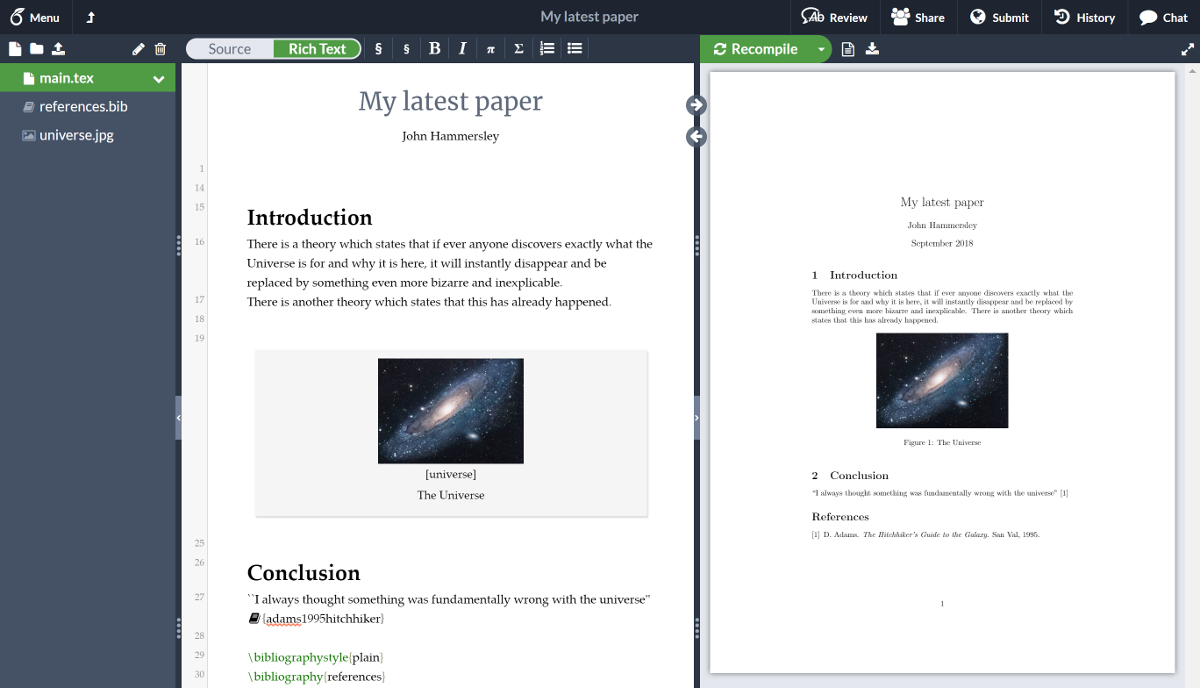
\includegraphics[scale=0.78]{figure/overleaf}
\end{frame}


\subsection{一点点经验分享}
\begin{frame}{一点经验分享}
	\begin{itemize}
		\item \LaTeX 是排版系统,不是文字处理器
		\item 所有文档都是过时的
		\item 请不要使用 CTeX套装发行版,使用\CTeX 宏包
		\item 如果要输入中文
		\begin{itemize}
			\item[*] 请用 XeLaTeX,请用 XeLaTeX,请用 XeLaTeX。
			\item[*] UTF-8编码,UTF-8编码,UTF-8编码。
		\end{itemize}
		\item 写一点编译一次,提高容错
		\item 用好百度,Google
	\end{itemize}
\end{frame}


\begin{frame}{参考文献}
	\beamertemplatetextbibitems 
	\bibliography{ref/refs}
\end{frame}

\begin{frame}
	\begin{itemize}
		\item 本幻灯片源码:
		\begin{itemize}
			\item \url{https://github.com/Neiou8/neepu-latex-talk}
		    \item 模板 \url{https://github.com/Neiou8/neepu-slides}
		\end{itemize}
		\item 本幻灯片基于:
		\begin{itemize}
			\item \url{https://github.com/tuna/thulib-latex-talk}
		\end{itemize}
		\item 许可证:CC BY-SA 4.0 Unported \ccbysa
	\end{itemize}
\end{frame}


\begin{frame}
	\centering \calligra \zihao{1} Thank you!
\end{frame}


\end{document}
